\chapter{Balanços termodinâmicos e sistemas abertos}\label{ch:b2:open-systems}

A termodinâmica do volume do primeiro ano tratou de sistemas fechados ---
uma massa fixa de gás num cilindro, comprimida, aquecida, expandida. Mas
as máquinas que de fato aquecem nossas casas, resfriam nossos alimentos e fazem nossa
eletricidade são atravessadas por um \emph{escoamento}: o vapor corre pela
turbina de uma usina a centenas de quilogramas por segundo, um
fluido refrigerante circula pelo compressor, pelo condensador, pela válvula e pelo
evaporador de uma bomba de calor, o ar passa pelo compressor e pela
câmara de combustão de um motor a jato. Cada componente é um \emph{\omterm{def:b2:open-systems:cv}{sistema
aberto}}, uma região do espaço com matéria entrando e saindo, e o
primeiro e o segundo princípios devem ser reescritos para ele. A reescrita é curta
--- o essencial é que o fluido empurrado para dentro do sistema carrega, além de
sua energia interna, o trabalho feito para empurrá-lo, razão pela qual
a \emph{\omterm{thm:b2:open-systems:firstlaw}{entalpia}}, e não a energia interna, é a energia natural de um escoamento.
Este capítulo estabelece os balanços de massa, energia e entropia para
\omterm{def:b2:open-systems:cv}{sistemas abertos} em \omterm{def:b2:open-systems:cv}{escoamento estacionário}, aplica-os aos dispositivos elementares ---
\omterm{prop:b2:open-systems:devices}{bocal}, válvula de \omterm{prop:b2:open-systems:devices}{estrangulamento}, compressor, turbina, \omterm{prop:b2:open-systems:devices}{trocador de calor} --- e reúne
esses dispositivos nos dois ciclos que o problema de fim de semana dimensiona: uma
bomba de calor e uma usina a vapor.

\begin{omfigure}
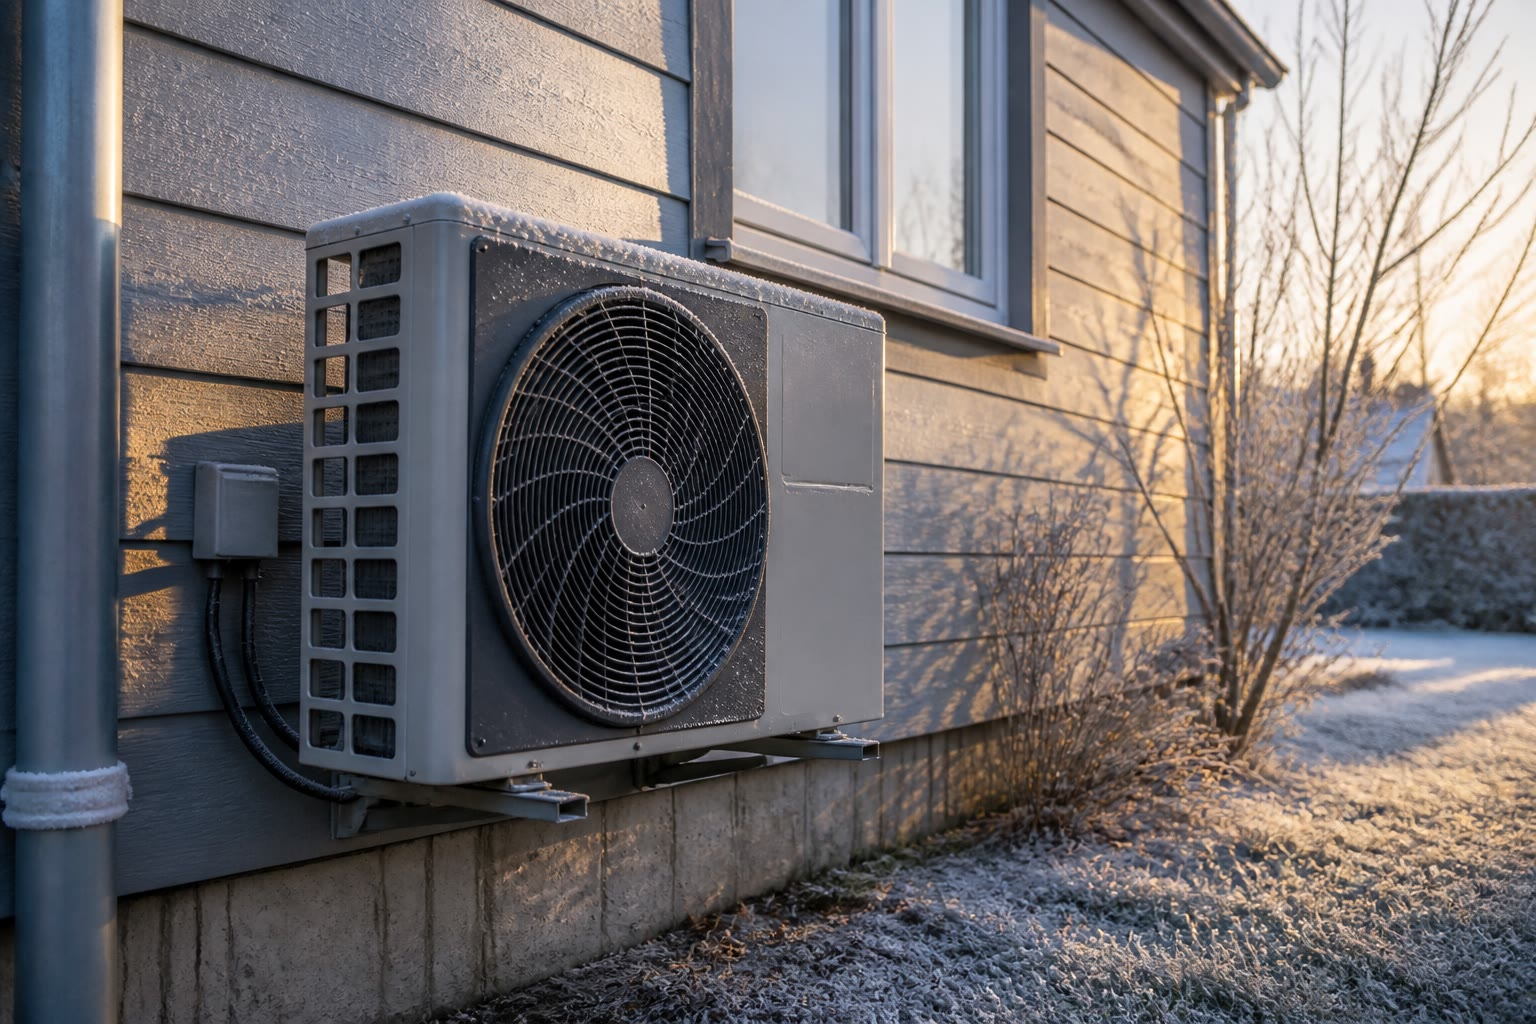
\includegraphics[width=0.58\linewidth]{images/book4/ai/b4-27-heat-pump-winter.jpg}

{\small A unidade externa de uma bomba de calor numa manhã de inverno: um ventilador
puxa o ar frio sobre o evaporador e, dentro, um compressor, um
condensador e uma válvula levam esse calor, multiplicado três ou quatro vezes,
para dentro da casa.}
\end{omfigure}

\section{Sistemas abertos e o balanço de massa}

\begin{definition}[Sistema aberto, volume de controle, escoamento estacionário]\label{def:b2:open-systems:cv}
Um \emph{sistema aberto}\index{sistema aberto} é uma região fixa do espaço,
o \emph{volume de controle}\index{volume de controle} $\Sigma$, limitado por uma
superfície através da qual o fluido entra e sai (seções de entrada e de
saída) e através da qual calor e trabalho podem ser trocados com o
exterior; o trabalho recebido por peças móveis (um eixo, um pistão)
que não sejam o próprio escoamento é o \emph{trabalho útil}\index{trabalho útil}
$W_{\text{u}}$ (trabalho de eixo). O escoamento é \emph{estacionário}\index{escoamento
estacionário} quando todo campo no interior de $\Sigma$ é independente do tempo: a massa,
a energia e a entropia contidas em $\Sigma$ são então constantes.
\end{definition}

\begin{proposition}[Balanço de massa]\label{prop:b2:open-systems:mass}
Através de uma seção de área $S$ em que o fluido de massa volúmica $\rho$ se move
à velocidade média $c$ normal a ela escoa a \emph{vazão
mássica}\index{vazão mássica} $\dot m = \rho c S$ (em \unit{kg/s}). Num
\omterm{def:b2:open-systems:cv}{escoamento estacionário}, o que entra sai: $\sum_{\text{in}}\dot m = \sum_{\text{out}}
\dot m$; para uma única corrente, $\dot m$ é a mesma na entrada e na saída,
$\rho_1c_1S_1 = \rho_2c_2S_2$ --- a \omterm{thm:b2:fluid-kinematics:continuity}{equação da continuidade} do
\cref{ch:b2:fluid-kinematics} integrada sobre a seção.
\end{proposition}

\begin{proof}
A massa em $\Sigma$ é constante, de modo que os fluxos se equilibram.
\end{proof}

\section{O primeiro princípio para um sistema aberto}

\begin{theorem}[Balanço de energia de um escoamento estacionário de uma corrente]\label{thm:b2:open-systems:firstlaw}
Para um \omterm{def:b2:open-systems:cv}{escoamento estacionário} de \omterm{def:b2:fluid-kinematics:flowrate}{vazão mássica} $\dot m$ que entra no estado 1
e sai no estado 2, recebendo a potência útil (de eixo)
$P_{\text{u}}$ e a potência térmica $P_{\text{th}}$,
\[
\dot m\,\Big[(h_2 - h_1) + \tfrac12(c_2^2 - c_1^2) + g(z_2 - z_1)\Big]
= P_{\text{u}} + P_{\text{th}} ,
\]
ou, por unidade de massa de fluido que atravessa o sistema,
\[
\Delta h + \Delta\big(\tfrac12c^2\big) + g\,\Delta z = w_{\text{u}} + q .
\]
A \emph{entalpia}\index{entalpia (num escoamento)} $h = u + Pv$ substitui
a energia interna: $Pv$ é o \emph{trabalho de escoamento}, o trabalho feito pelo
fluido a montante para empurrar uma unidade de massa para dentro, menos o feito para empurrá-la
para fora.
\end{theorem}

\begin{proof}
Siga o sistema fechado formado pelo fluido dentro de $\Sigma$ em $t$ mais
a porção $\dd m = \dot m\,\dd t$ prestes a entrar; em $t + \dd t$ ele
consiste no fluido dentro de $\Sigma$ (mesmo estado, \omterm{def:b2:open-systems:cv}{estacionário}) mais a
porção $\dd m$ que saiu. Sua energia variou de
$\dd m\,[(u_2 + \tfrac12c_2^2 + gz_2) - (u_1 + \tfrac12c_1^2 + gz_1)]$. Ele
recebeu $P_{\text{u}}\dd t + P_{\text{th}}\dd t$, mais o trabalho das
forças de pressão na entrada, $P_1S_1 \times c_1\dd t = P_1v_1\,\dd m$
(que empurra a porção para dentro), menos o da saída, $P_2v_2\,\dd m$. O
primeiro princípio para esse sistema fechado, com $u + Pv = h$, dá o resultado.
\end{proof}

\begin{omfigure}
\begin{tikzpicture}[scale=0.95, >=stealth]
  \draw[thick, rounded corners=6pt, fill=omDef!8] (1.2,0) rectangle (6.2,2.6);
  \node[font=\scriptsize] at (3.7,1.9) {volume de controle $\Sigma$ (estacionário)};
  % tubo de entrada
  \draw[thick] (-0.6,0.5) -- (1.2,0.5); \draw[thick] (-0.6,1.1) -- (1.2,1.1);
  \fill[omExo!40] (-0.5,0.52) rectangle (0.1,1.08);
  \node[font=\scriptsize, above] at (-0.2,1.12) {$\dd m$};
  \draw[->, omExo, thick] (-1.4,0.8) -- (-0.6,0.8);
  \node[font=\scriptsize, left] at (-1.4,0.8) {$\dot m$, $h_1$, $c_1$, $z_1$};
  % tubo de saída
  \draw[thick] (6.2,1.5) -- (8.0,1.5); \draw[thick] (6.2,2.1) -- (8.0,2.1);
  \fill[omExo!40] (7.3,1.52) rectangle (7.9,2.08);
  \node[font=\scriptsize, above] at (7.6,2.12) {$\dd m$};
  \draw[->, omExo, thick] (8.0,1.8) -- (8.8,1.8);
  \node[font=\scriptsize, right] at (8.8,1.8) {$h_2$, $c_2$, $z_2$};
  % eixo
  \draw[->, omThm, very thick] (3.7,-0.8) -- (3.7,0) node[pos=0, below, font=\scriptsize] {$P_{\text{u}}$ (eixo)};
  \draw[->, omThm, very thick] (5.5,3.4) -- (5.5,2.6) node[pos=0, above, font=\scriptsize] {$P_{\text{th}}$};
  % empurrões de pressão
  \node[font=\scriptsize, omExo] at (0.3,0.2) {$P_1v_1$ empurra para dentro};
  \node[font=\scriptsize, omExo] at (7.2,1.2) {$P_2v_2$ empurra para fora};
\end{tikzpicture}

{\small O \omterm{def:b2:open-systems:cv}{sistema aberto} \omterm{def:b2:open-systems:cv}{estacionário}: o sistema fechado seguido durante $\dd
t$ é o conteúdo de $\Sigma$ mais a porção que entra, depois o conteúdo
mais a porção que sai; o trabalho de pressão nas duas seções transforma $u$
em $h = u + Pv$.}
\end{omfigure}

\begin{remark}[Usar o primeiro princípio]\label{rem:b2:open-systems:using}
Para um gás perfeito $\Delta h = c_p\Delta T$; para um líquido $\Delta h \approx
c\,\Delta T + v\,\Delta P$ (o segundo termo é o trabalho da bomba); para um vapor
lê-se $h$ em tabelas ou diagramas. O termo cinético em geral é
desprezível: a \qty{10}{m/s}, $c^2/2 = \qty{50}{J/kg}$, contra
\qty{1}{kJ/kg} para um kelvin de ar --- ele só importa em bocais e
em pás de turbina, onde as velocidades chegam a centenas de metros por segundo. O
termo potencial, $g\Delta z \approx \qty{10}{J/kg}$ por metro, importa para a
água numa barragem, nunca num ciclo a gás. Com várias entradas e saídas
o balanço se escreve $\sum_{\text{out}}\dot m\,h - \sum_{\text{in}}\dot m\,h =
P_{\text{u}} + P_{\text{th}}$ (termos cinético e potencial desprezados).
\end{remark}

\section{O segundo princípio para um sistema aberto}

\begin{theorem}[Balanço de entropia de um escoamento estacionário]\label{thm:b2:open-systems:secondlaw}
Para um \omterm{def:b2:open-systems:cv}{escoamento estacionário} de uma corrente que troca as potências térmicas
$P_{\text{th},i}$ com fontes às temperaturas $T_i$,
\[
\dot m\,(s_2 - s_1) = \sum_i\frac{P_{\text{th},i}}{T_i} + \dot S_{\text{c}},
\qquad \dot S_{\text{c}} \ge 0 ;
\]
por unidade de massa, $\Delta s = s_{\text{troc}} + s_{\text{c}}$. Um escoamento
adiabático e reversível é \emph{isentrópico}; um escoamento adiabático real tem $s_2 >
s_1$. O \emph{rendimento isentrópico}\index{rendimento isentrópico} de
uma turbina é $\eta_{\text{T}} = w_{\text{real}}/w_{\text{s}} = (h_1 - h_2)/(h_1
- h_{2s})$ e o de um compressor $\eta_{\text{C}} = (h_{2s} - h_1)/(h_2 -
h_1)$, onde $2s$ é o estado alcançado isentropicamente à mesma
pressão de saída; ambos valem tipicamente $0.8$--$0.9$. O trabalho perdido pela
irreversibilidade, referido à temperatura ambiente $T_0$, vale
$T_0\,s_{\text{c}}$ por unidade de massa.
\end{theorem}

\begin{proof}
O mesmo sistema fechado de antes: sua entropia varia de $\dd m\,(s_2 -
s_1)$, ele recebe $\sum P_{\text{th},i}\dd t/T_i$ das fontes, e o
resto é criado.
\end{proof}

\section{Os dispositivos elementares}

\begin{proposition}[Bocal, estrangulamento, compressor, turbina, trocador]\label{prop:b2:open-systems:devices}
Todos adiabáticos salvo menção contrária, \omterm{def:b2:open-systems:cv}{estacionários}, com os termos cinético e potencial
desprezados a menos que sejam o ponto em questão.
\begin{itemize}
\item \emph{Bocal}\index{bocal} (sem eixo, sem calor): $\tfrac12c_2^2 -
      \tfrac12c_1^2 = h_1 - h_2$ --- a \omterm{thm:b2:open-systems:firstlaw}{entalpia} vira velocidade; um
      \emph{difusor} faz o contrário.
\item \emph{Estrangulamento}\index{estrangulamento} (válvula, tampão poroso; sem eixo,
      sem calor, velocidades pequenas): $h_2 = h_1$, \emph{isentálpico}. Para um
      gás perfeito $T_2 = T_1$; para um gás real a temperatura em geral
      cai (efeito Joule--Thomson); para um líquido perto da saturação uma
      fração vaporiza bruscamente --- a válvula de expansão de todo
      refrigerador.
\item \emph{Compressor, bomba, turbina}\index{turbina} (máquinas
      adiabáticas): $w_{\text{u}} = h_2 - h_1$ --- positivo para um compressor,
      negativo para uma turbina; para uma bomba de líquido $w_{\text{u}} \approx
      v(P_2 - P_1)$, minúsculo porque $v$ é pequeno.
\item \emph{Trocador de calor}\index{trocador de calor} (duas correntes, sem
      eixo, adiabático como um todo): $\dot m_{\text{a}}(h_{\text{a},2} -
      h_{\text{a},1}) = -\dot m_{\text{b}}(h_{\text{b},2} - h_{\text{b},1})$
      --- o que um perde o outro ganha; a troca cria entropia
      a menos que as correntes estejam à mesma temperatura em toda parte
      (a contracorrente a reduz).
\item \emph{Câmara de mistura}: $\sum\dot m_{\text{in}}h_{\text{in}} = \dot
      m_{\text{out}}h_{\text{out}}$.
\end{itemize}
\end{proposition}

\begin{proof}
Cada um é o primeiro princípio com os termos apropriados anulados.
\end{proof}

\begin{omfigure}
\begin{tikzpicture}[scale=0.85, >=stealth]
  % bocal
  \draw[thick] (0,0.2) -- (1.6,0.55) -- (1.6,0.85) -- (0,1.2);
  \draw[->, omExo, thick] (-0.6,0.7) -- (-0.1,0.7);
  \draw[->, omExo, very thick] (1.7,0.7) -- (2.9,0.7);
  \node[font=\scriptsize] at (1.0,-0.35) {bocal: $h \to c^2/2$};
  % estrangulamento
  \begin{scope}[xshift=4.6cm]
    \draw[thick] (0,0.4) -- (1.0,0.4) -- (1.0,0.55) -- (1.2,0.55) -- (1.2,0.4) -- (2.4,0.4);
    \draw[thick] (0,1.0) -- (1.0,1.0) -- (1.0,0.85) -- (1.2,0.85) -- (1.2,1.0) -- (2.4,1.0);
    \draw[->, omExo, thick] (-0.6,0.7) -- (-0.1,0.7);
    \draw[->, omExo, thick] (2.5,0.7) -- (3.1,0.7);
    \node[font=\scriptsize] at (1.2,-0.35) {estrangulamento: $h_2 = h_1$};
    \node[font=\scriptsize] at (0.4,1.3) {$P_1$}; \node[font=\scriptsize] at (2.0,1.3) {$P_2 < P_1$};
  \end{scope}
  % turbina
  \begin{scope}[xshift=9.6cm]
    \draw[thick] (0,1.3) -- (0,0.1) -- (2.0,-0.3) -- (2.0,1.7) -- cycle;
    \draw[->, omExo, thick] (-0.7,1.0) -- (-0.1,1.0);
    \draw[->, omExo, thick] (2.1,0.3) -- (2.8,0.3);
    \draw[->, omThm, very thick] (1.0,-0.4) -- (1.0,-1.0) node[below, font=\scriptsize] {$w_{\text{u}} = h_2 - h_1 < 0$};
    \node[font=\scriptsize] at (1.0,2.0) {turbina};
  \end{scope}
  % trocador
  \begin{scope}[yshift=-3.2cm]
    \draw[thick, rounded corners=4pt] (0,0) rectangle (4.4,1.4);
    \draw[->, omExo, very thick] (-0.6,1.1) -- (0,1.1); \draw[omExo, very thick] (0,1.1) -- (4.4,1.1); \draw[->, omExo, very thick] (4.4,1.1) -- (5.0,1.1);
    \draw[<-, omDef, very thick] (-0.6,0.3) -- (0,0.3); \draw[omDef, very thick] (0,0.3) -- (4.4,0.3); \draw[<-, omDef, very thick] (4.4,0.3) -- (5.0,0.3);
    \node[font=\scriptsize, omExo, left] at (-0.6,1.1) {quente entra}; \node[font=\scriptsize, omExo, right] at (5.0,1.1) {quente sai};
    \node[font=\scriptsize, omDef, right] at (5.0,0.3) {frio entra}; \node[font=\scriptsize, omDef, left] at (-0.6,0.3) {frio sai};
    \node[font=\scriptsize] at (2.2,-0.4) {trocador em contracorrente: $\dot m_{\text{a}}\Delta h_{\text{a}} = -\dot m_{\text{b}}\Delta h_{\text{b}}$};
    \node[font=\scriptsize] at (8.4,0.7) {(a câmara de mistura: $\sum\dot m_{\text{in}}h_{\text{in}} = \dot m_{\text{out}}h_{\text{out}}$)};
  \end{scope}
\end{tikzpicture}

{\small Os \omterm{def:b2:open-systems:cv}{sistemas abertos} elementares: cada um é o balanço de energia com
os termos irrelevantes riscados --- sem eixo num \omterm{prop:b2:open-systems:devices}{bocal} ou num \omterm{prop:b2:open-systems:devices}{estrangulamento},
sem calor numa turbina adiabática, sem calor líquido num trocador tomado como
um todo.}
\end{omfigure}

\begin{example}[Números para os dispositivos]\label{ex:b2:open-systems:numbers}
Vapor que entra no \omterm{prop:b2:open-systems:devices}{bocal} de uma turbina com $h = \qty{3000}{kJ/kg}$ e sai
com \qty{2800}{kJ/kg} atinge $c = \sqrt{2 \times 200 \times 10^3} =
\qty{630}{m/s}$. Ar comprimido adiabaticamente de \qty{1}{bar},
\qty{293}{K} a \qty{8}{bar}: isentropicamente $T_2 = 293 \times 8^{0.286} =
\qty{531}{K}$ e $w = c_p\Delta T = \qty{239}{kJ/kg}$; com $\eta_{\text{C}} =
0.8$, \qty{299}{kJ/kg} e \qty{590}{K} --- razão pela qual os compressores são
resfriados entre estágios. Um radiador de carro que retira \qty{42}{kW} da água
resfriada de \qty{10}{K} (\qty{1}{kg/s}) aquece \qty{2.1}{kg/s} de ar de
\qty{20}{K}. Refrigerante líquido a \qty{40}{\celsius} estrangulado até
\qty{0}{\celsius} chega como uma névoa com $28\%$ de vapor: essa vaporização brusca
é o que resfria o líquido até a temperatura do evaporador.
\end{example}

\section{Ciclos}

\begin{proposition}[Refrigeração por compressão de vapor e bomba de calor]\label{prop:b2:open-systems:fridge}
Um fluido refrigerante circula por: (1$\to$2) um compressor adiabático
que eleva o vapor da pressão do evaporador à pressão do
condensador, $w = h_2 - h_1$; (2$\to$3) um condensador em que ele libera
$q_{\text{cond}} = h_2 - h_3$ para o lado quente (a sala, para uma bomba de calor; a
cozinha, para uma geladeira) e sai como líquido; (3$\to$4) um \omterm{prop:b2:open-systems:devices}{estrangulamento}, $h_4
= h_3$; (4$\to$1) um evaporador em que ele absorve $q_{\text{evap}} = h_1 - h_4$
do lado frio. Os coeficientes de desempenho valem
\[
\mathrm{COP}_{\text{frio}} = \frac{h_1 - h_4}{h_2 - h_1}, \qquad
\mathrm{COP}_{\text{quente}} = \frac{h_2 - h_3}{h_2 - h_1} = \mathrm{COP}_{\text{frio}} + 1 ,
\]
limitados pelos de Carnot, $T_{\text{c}}/(T_{\text{h}} - T_{\text{c}})$ e
$T_{\text{h}}/(T_{\text{h}} - T_{\text{c}})$; o ciclo se lê mais facilmente no
diagrama $(\log P, h)$, em que as duas trocas e o trabalho são
segmentos horizontais.
\end{proposition}

\begin{proof}
Os quatro balanços do primeiro princípio; o balanço de energia de todo o ciclo
dá $q_{\text{cond}} = q_{\text{evap}} + w$, e daí a relação entre
os dois COP.
\end{proof}

\begin{omfigure}
\begin{tikzpicture}
  \begin{axis}[width=8.6cm, height=5.2cm, xmin=150, xmax=480, ymin=-0.1, ymax=1.5,
    axis x line=bottom, axis y line=left, xlabel={$h$ (\unit{kJ/kg})}, ylabel={$\log P$},
    xlabel style={at={(axis description cs:0.5,-0.12)}, anchor=north}, ytick=\empty, xtick={200,300,400}, clip=false]
    % domo de saturação (esquemático)
    \addplot[gray, thick, smooth] coordinates {(200,0.3) (215,0.55) (232,0.85) (256,1.1) (290,1.3) (330,1.38) (370,1.3) (405,1.1) (418,0.85) (418,0.55) (399,0.3)};
    % ciclo
    \draw[omDef, very thick] (axis cs:256,1.1) -- (axis cs:256,0.3);
    \draw[omDef, very thick] (axis cs:256,0.3) -- (axis cs:399,0.3);
    \draw[omDef, very thick] (axis cs:399,0.3) -- (axis cs:433,1.1);
    \draw[omDef, very thick] (axis cs:433,1.1) -- (axis cs:256,1.1);
    \fill (axis cs:399,0.3) circle (1.5pt) node[below, font=\scriptsize] {1};
    \fill (axis cs:433,1.1) circle (1.5pt) node[above, font=\scriptsize] {2};
    \fill (axis cs:256,1.1) circle (1.5pt) node[above, font=\scriptsize] {3};
    \fill (axis cs:256,0.3) circle (1.5pt) node[below, font=\scriptsize] {4};
    \node[font=\scriptsize, omDef] at (axis cs:330,0.2) {evaporador $q_{\text{evap}}$};
    \node[font=\scriptsize, omDef] at (axis cs:345,1.2) {condensador $q_{\text{cond}}$};
    \node[font=\scriptsize, omDef, anchor=west] at (axis cs:418,0.68) {$w$};
    \node[font=\scriptsize, gray] at (axis cs:205,0.95) {líquido};
    \node[font=\scriptsize, gray] at (axis cs:450,0.5) {vapor};
    \node[font=\scriptsize, gray] at (axis cs:330,0.75) {líquido + vapor};
  \end{axis}
\end{tikzpicture}

{\small O ciclo de compressão de vapor no diagrama $(\log P, h)$: o
condensador e o evaporador são isóbaras dentro do domo, o \omterm{prop:b2:open-systems:devices}{estrangulamento} uma
isentálpica vertical, o compressor uma linha inclinada; os comprimentos dos
segmentos horizontais são os calores e o trabalho por quilograma.}
\end{omfigure}

\begin{proposition}[O ciclo a vapor (de Rankine)]\label{prop:b2:open-systems:rankine}
A água circula por: (1$\to$2) uma bomba, $w_{\text{p}} \approx v(P_2 -
P_1)$, alguns \unit{kJ/kg}; (2$\to$3) uma caldeira em alta pressão em que ela
é aquecida, vaporizada e superaquecida, $q_{\text{in}} = h_3 - h_2$;
(3$\to$4) uma turbina que expande o vapor até a pressão do condensador,
$w_{\text{t}} = h_3 - h_4$ (mil \unit{kJ/kg}); (4$\to$1) um condensador
em baixa pressão em que o vapor úmido volta a ser líquido, rejeitando
$q_{\text{out}} = h_4 - h_1$ à água de refrigeração. O rendimento vale
\[
\eta = \frac{w_{\text{t}} - w_{\text{p}}}{q_{\text{in}}} = 1 - \frac{q_{\text{out}}}{q_{\text{in}}} ,
\]
cerca de $0.35$--$0.45$ na prática; o calor é fornecido a uma
temperatura média $\bar T = q_{\text{in}}/(s_3 - s_2)$ bem abaixo do
pico da caldeira, razão pela qual o superaquecimento, o reaquecimento e as pressões altas elevam
$\eta$, e razão pela qual a exaustão deve permanecer seca o bastante ($x_4 \gtrsim 0.88$) para
poupar as últimas pás da erosão por gotículas.
\end{proposition}

\begin{proof}
Primeiro princípio em cada componente, depois no ciclo: $w_{\text{t}} - w_{\text{p}}
= q_{\text{in}} - q_{\text{out}}$.
\end{proof}

\begin{omfigure}
\begin{tikzpicture}
  \begin{axis}[width=8.4cm, height=5.2cm, xmin=0, xmax=9.5, ymin=250, ymax=820,
    axis x line=bottom, axis y line=left, xlabel={$s$ (\unit{kJ/kg/K})}, ylabel={$T$ (\unit{K})},
    xlabel style={at={(axis description cs:0.5,-0.12)}, anchor=north}, xtick={2,4,6,8}, ytick={300,500,700}, clip=false]
    % domo
    \addplot[gray, thick, smooth] coordinates {(0.4,280) (1.3,373) (2.3,473) (3.3,560) (4.4,647) (5.5,600) (6.3,520) (7.1,440) (7.9,373) (8.4,306)};
    % ciclo: 1 (0.48,306) 2 (0.5,308) ao longo do líquido saturado até 549K (3.1,549), vaporização até (5.9,549), superaquecimento até 3 (6.88,773); expansão até 4 (7.53,306); volta a 1
    \draw[omDef, very thick] (axis cs:0.48,306) -- (axis cs:0.5,309);
    \draw[omDef, very thick, smooth] plot coordinates {(0.5,309) (1.2,373) (2.2,470) (3.1,549)};
    \draw[omDef, very thick] (axis cs:3.1,549) -- (axis cs:5.9,549);
    \draw[omDef, very thick, smooth] plot coordinates {(5.9,549) (6.3,620) (6.88,773)};
    \draw[omDef, very thick] (axis cs:6.88,773) -- (axis cs:7.53,306);
    \draw[omDef, very thick, dashed] (axis cs:6.88,773) -- (axis cs:6.88,306);
    \draw[omDef, very thick] (axis cs:7.53,306) -- (axis cs:0.48,306);
    \fill (axis cs:0.48,306) circle (1.5pt) node[below left, font=\scriptsize] {1,2};
    \fill (axis cs:6.88,773) circle (1.5pt) node[above, font=\scriptsize] {3};
    \fill (axis cs:7.53,306) circle (1.5pt) node[below, font=\scriptsize] {4};
    \fill (axis cs:6.88,306) circle (1.5pt) node[below, font=\scriptsize] {4s};
    \node[font=\scriptsize, omDef] at (axis cs:3.8,600) {caldeira};
    \node[font=\scriptsize, omDef, anchor=west] at (axis cs:7.3,560) {turbina};
    \node[font=\scriptsize, omDef] at (axis cs:4.0,285) {condensador};
  \end{axis}
\end{tikzpicture}

{\small O ciclo de Rankine no diagrama $(T,s)$: bomba (invisível),
aquecimento ao longo da linha do líquido, vaporização à pressão da caldeira,
superaquecimento, expansão (isentrópica tracejada, real em traço cheio, terminando mais úmida ou
mais seca), condensação. É a temperatura média de fornecimento de calor, e não o
pico, que fixa o rendimento.}
\end{omfigure}

\begin{remark}[Outros ciclos, e um transitório]\label{rem:b2:open-systems:other}
A turbina a gás (compressor, câmara de combustão, turbina: o ciclo de
Brayton) tem o rendimento ideal $1 - r^{-(\gamma-1)/\gamma}$ para a
razão de pressões $r$ e rejeita sua exaustão a várias centenas de graus;
alimentar com essa exaustão um ciclo a vapor (ciclo combinado) chega a $60\%$.
Os \omterm{def:b2:open-systems:cv}{sistemas abertos} também têm transitórios: encher um tanque rígido evacuado a partir de
uma linha a $T_0$ termina em $T = \gamma T_0$ (o trabalho de escoamento $Pv$ vira
energia interna), \qty{120}{K} mais quente para o ar --- a razão pela qual um cilindro de
mergulho esquenta ao ser enchido.
\end{remark}

\begin{method}[Balanços de sistemas abertos]\label{meth:b2:open-systems:method}
(1) Desenhe o \omterm{def:b2:open-systems:cv}{volume de controle}; liste entradas, saídas, eixo e calor.
(2) Massa: $\sum\dot m_{\text{in}} = \sum\dot m_{\text{out}}$. (3) Energia
por unidade de massa: $\Delta h + \Delta c^2/2 + g\Delta z = w_{\text{u}} + q$, com
$\Delta h = c_p\Delta T$ para gases, tabelas para vapores, $v\Delta P$ para
bombas. (4) Entropia: $\Delta s = \sum q_i/T_i + s_{\text{c}}$, estados de
referência isentrópicos, rendimentos, $T_0s_{\text{c}}$ perdido. (5) Ciclos: leia
o diagrama, some ao longo da malha, compare com Carnot.
\end{method}

\section{Exercícios}

\begin{exercise}[$\star$]\label{exo:b2:open-systems:1}
(a) Uma mangueira de jardim entrega \qty{12}{L/min} por um \omterm{prop:b2:open-systems:devices}{bocal} de \qty{1}{cm}:
velocidade de saída. (b) Água quente a \qty{60}{\celsius}, \qty{0.1}{kg/s},
se mistura com água fria a \qty{10}{\celsius}, \qty{0.2}{kg/s}: temperatura
de saída. (c) Por que a mistura é irreversível --- calcule a
entropia criada por segundo.
\end{exercise}

\begin{exercise}[$\star$]\label{exo:b2:open-systems:2}
Vapor entra num \omterm{prop:b2:open-systems:devices}{bocal} a \qty{50}{m/s} com $h = \qty{3000}{kJ/kg}$ e
sai com \qty{2800}{kJ/kg}: velocidade de saída. Ar a \qty{300}{K} acelerado
do repouso a \qty{300}{m/s} num \omterm{prop:b2:open-systems:devices}{bocal} ($c_p = \qty{1005}{J/kg/K}$):
queda de temperatura. Um difusor freia o ar de \qty{250}{m/s} até o repouso: aumento.
\end{exercise}

\begin{exercise}[$\star$]\label{exo:b2:open-systems:3}
\omterm{prop:b2:open-systems:devices}{Estrangulamento}. (a) Um gás perfeito: o que acontece com $T$, com $s$? (b) Vapor úmido
a \qty{10}{bar} ($h_{\text{f}} = 763$, $h_{\text{fg}} = \qty{2015}{kJ/kg}$),
título $0.9$, estrangulado até \qty{1}{bar} ($h_{\text{f}} = 417$, $h_{\text{fg}}
= \qty{2258}{kJ/kg}$): título final --- o calorímetro de \omterm{prop:b2:open-systems:devices}{estrangulamento}. (c)
Refrigerante líquido a \qty{40}{\celsius} ($h = \qty{256}{kJ/kg}$) estrangulado
até \qty{0}{\celsius} ($h_{\text{f}} = 200$, $h_{\text{g}} = \qty{399}{kJ/kg}$):
fração de vapor.
\end{exercise}

\begin{exercise}[$\star$]\label{exo:b2:open-systems:4}
(a) Um radiador resfria \qty{1}{kg/s} de água de \qty{90}{} a \qty{80}{\celsius};
o ar ($c_p = \qty{1005}{J/kg/K}$) esquenta de \qty{20}{} a \qty{40}{\celsius}:
\omterm{def:b2:fluid-kinematics:flowrate}{vazão mássica} e \omterm{def:b2:fluid-kinematics:flowrate}{vazão volumétrica} de ar. (b) Uma turbina a vapor, \qty{10}{kg/s},
com $h$ de \qty{3400}{} a \qty{2400}{kJ/kg}: potência. (c) Uma bomba eleva a
água de \qty{1}{} a \qty{60}{bar}: trabalho por quilograma, e potência para
\qty{500}{kg/s}.
\end{exercise}

\begin{exercise}[$\star\star$]\label{exo:b2:open-systems:5}
\emph{O trabalho de escoamento.} (a) Refaça a dedução do primeiro princípio para \omterm{def:b2:open-systems:cv}{sistemas abertos} e
explique de onde vem $Pv$. (b) Por que a energia interna $u$
aparece num sistema fechado e $h$ num escoamento? (c) Compare $c^2/2$ a
\qty{10}{m/s} e a \qty{300}{m/s} com $c_p\Delta T$ para \qty{1}{K} de ar.
(d) Água que cai \qty{100}{m} por um conduto forçado: $g\Delta z$ contra
$c\,\Delta T$ para \qty{1}{K}; conclua quanto a água esquenta se a
turbina for retirada.
\end{exercise}

\begin{exercise}[$\star\star$]\label{exo:b2:open-systems:6}
\emph{Compressores.} Ar, \qty{1}{bar}, \qty{293}{K}, até \qty{8}{bar}; $\gamma =
1.4$, $c_p = \qty{1005}{J/kg/K}$, $r = \qty{287}{J/kg/K}$. (a) Temperatura
isentrópica de saída e trabalho. (b) Com $\eta_{\text{C}} = 0.8$: trabalho, temperatura
de saída, entropia criada. (c) Dois estágios de razão $\sqrt8$ com
resfriamento de volta a \qty{293}{K} entre eles: trabalho economizado. (d) Limite
isotérmico $rT\ln 8$; por que os compressores reais se aproximam dele com muitos estágios.
\end{exercise}

\begin{exercise}[$\star\star$]\label{exo:b2:open-systems:7}
\emph{Turbina.} Vapor a \qty{60}{bar}, \qty{500}{\celsius}: $h_3 = \qty{3422}{kJ/kg}$,
$s_3 = \qty{6.88}{kJ/kg/K}$; condensador a \qty{0.05}{bar} (\qty{33}{\celsius}):
$s_{\text{f}} = 0.476$, $s_{\text{g}} = \qty{8.394}{kJ/kg/K}$, $h_{\text{f}} = 138$,
$h_{\text{fg}} = \qty{2423}{kJ/kg}$. (a) Título e \omterm{thm:b2:open-systems:firstlaw}{entalpia} de saída
isentrópicos, trabalho. (b) Com $\eta_{\text{T}} = 0.85$: trabalho, \omterm{thm:b2:open-systems:firstlaw}{entalpia} e
título de saída. (c) Entropia criada por quilograma e trabalho perdido a $T_0 =
\qty{306}{K}$. (d) Por que uma exaustão úmida demais é um problema.
\end{exercise}

\begin{exercise}[$\star\star$]\label{exo:b2:open-systems:8}
\emph{Bomba de calor.} Evaporador a \qty{0}{\celsius}, condensador a \qty{40}{\celsius};
$h_1 = 399$ (vapor saturado, \qty{0}{\celsius}), $h_{2s} = 426$, $h_3 = 256$,
$h_4 = h_3$ (\unit{kJ/kg}); $\eta_{\text{C}} = 0.8$. (a) $h_2$ e o trabalho.
(b) Calores trocados, os dois COP. (c) COP de Carnot; razão. (d) \omterm{def:b2:fluid-kinematics:flowrate}{Vazão mássica}
e potência elétrica para \qty{8}{kW} de aquecimento; por que o COP cai quando
o ar externo esfria.
\end{exercise}

\begin{exercise}[$\star\star$]\label{exo:b2:open-systems:9}
\emph{Entropia num trocador.} Água quente a \qty{1}{kg/s} de \qty{90}{} a
\qty{50}{\celsius} aquece água fria a \qty{2}{kg/s} a partir de \qty{10}{\celsius}.
(a) Temperatura de saída da corrente fria. (b) Entropia criada por
segundo ($c = \qty{4180}{J/kg/K}$). (c) Potência perdida a $T_0 = \qty{293}{K}$,
comparada com os \qty{167}{kW} trocados. (d) Por que um arranjo em
corrente paralela criaria mais entropia que a contracorrente para o mesmo serviço?
\end{exercise}

\begin{exercise}[$\star\star\star$]\label{exo:b2:open-systems:10}
\emph{Encher um tanque.} Um tanque rígido, evacuado e isolado é ligado
a uma linha que transporta um gás perfeito a $T_0$, $P_0$. (a) Escreva o balanço
de energia do tanque durante o enchimento (não \omterm{def:b2:open-systems:cv}{estacionário}: sua energia cresce) e
mostre que o gás em seu interior termina a $T = \gamma T_0$. (b) Ar a \qty{293}{K}:
temperatura final. (c) Se o tanque contivesse inicialmente gás a $T_0$ e
$P_1 < P_0$, argumente que a temperatura final fica entre $T_0$ e
$\gamma T_0$. (d) Por que um cilindro de mergulho esquenta ao ser enchido, e por que
ele é enchido lentamente dentro da água?
\end{exercise}

\begin{exercise}[$\star\star\star$]\label{exo:b2:open-systems:11}
\emph{Reaquecimento.} A turbina do \cref{exo:b2:open-systems:7} é dividida:
expansão até \qty{10}{bar} (fim isentrópico: $h = \qty{2850}{kJ/kg}$), reaquecimento
a \qty{500}{\celsius} ($h = 3478$, $s = \qty{7.76}{kJ/kg/K}$), expansão até
\qty{0.05}{bar}, os dois estágios isentrópicos. Trabalho da bomba \qty{6}{kJ/kg}, $h_2 =
\qty{144}{kJ/kg}$. (a) Título e \omterm{thm:b2:open-systems:firstlaw}{entalpia} de saída do segundo estágio. (b)
Trabalho e calor totais; rendimento; compare com a expansão única
($\eta = 0.40$ isentrópico). (c) Por que o reaquecimento ajuda, em termos da
temperatura média de fornecimento de calor? (d) O que mais ele resolve?
\end{exercise}

\begin{exercise}[$\star\star\star$]\label{exo:b2:open-systems:12}
\emph{Turbina a gás e ciclo combinado.} Ar comprimido isentropicamente
de \qty{1}{bar}, \qty{293}{K} a \qty{12}{bar}, aquecido a pressão constante
até \qty{1500}{K}, expandido isentropicamente até \qty{1}{bar}; $\gamma = 1.4$,
$c_p = \qty{1005}{J/kg/K}$. (a) As quatro temperaturas. (b) Trabalhos,
calor, rendimento; mostre que $\eta = 1 - r^{-(\gamma - 1)/\gamma}$. (c) A
exaustão a $T_4$ gera vapor para um ciclo de Rankine de rendimento $0.35$
que recupera $70\%$ do calor da exaustão acima de \qty{373}{K}: rendimento
combinado. (d) Por que o ciclo combinado é a usina térmica mais eficiente
que existe?
\end{exercise}

\section{Problema: uma bomba de calor doméstica e uma usina a vapor}

\begin{problem}[{Problema de fim de semana --- duas máquinas dimensionadas com os
balanços de sistemas abertos}]\label{pb:b2:open-systems:1}
\textbf{Parte I --- A bomba de calor.}
Dados do refrigerante (\unit{kJ/kg}, \unit{kJ/kg/K}): vapor saturado a
\qty{0}{\celsius} ($P = \qty{2.9}{bar}$): $h_1 = 399$, $s_1 = 1.727$;
líquido saturado a \qty{0}{\celsius}: $h_{\text{f}} = 200$, $s_{\text{f}} = 1.00$;
à pressão do condensador \qty{10.2}{bar} ($T_{\text{sat}} = \qty{40}{\celsius}$):
fim da compressão isentrópica $h_{2s} = 426$, líquido saturado $h_3 = 256$,
$s_3 = 1.19$; o vapor superaquecido ali tem $c_p \approx \qty{1.0}{kJ/kg/K}$.
Compressor com $\eta_{\text{C}} = 0.8$; demanda da casa \qty{8}{kW}.
\begin{enumerate}
  \item Esboce o ciclo num diagrama $(\log P, h)$ e nomeie os quatro
        componentes com o processo que cada um realiza.
  \item Estado 4 após o \omterm{prop:b2:open-systems:devices}{estrangulamento}: \omterm{thm:b2:open-systems:firstlaw}{entalpia} e fração de vapor.
  \item Calor absorvido por quilograma no evaporador.
  \item Trabalho do compressor, isentrópico e real; $h_2$ e uma estimativa de
        $T_2$.
  \item Calor liberado no condensador; os dois COP; verifique a
        relação entre eles.
  \item COP de Carnot entre \qty{0}{} e \qty{40}{\celsius}; que
        fração a máquina atinge?
  \item \omterm{def:b2:fluid-kinematics:flowrate}{Vazão mássica} de refrigerante e potência elétrica (rendimento
        do motor $0.9$).
  \item Entropia criada por quilograma no compressor e no
        \omterm{prop:b2:open-systems:devices}{estrangulamento} ($s_4 = s_{\text{f}} + x\,(s_1 - s_{\text{f}})$); qual é
        o pior?
\end{enumerate}

\textbf{Parte II --- Tempo frio e escolhas de projeto.}
\begin{enumerate}[resume]
  \item A \qty{-10}{\celsius} lá fora, o evaporador funciona a
        \qty{-15}{\celsius}: COP de Carnot para aquecimento; por que o COP
        real cai mais depressa (pense na razão de pressões e na
        densidade do vapor)?
  \item Por que se forma geada na serpentina externa, e quanto custa o
        ciclo de degelo?
  \item Aquecimento de piso a \qty{35}{\celsius} contra radiadores a
        \qty{55}{\celsius}: COP de Carnot com o evaporador a
        \qty{0}{\celsius}; conclua.
  \item Compare, por quilowatt-hora de combustível queimado numa usina de
        rendimento $0.40$, o calor entregue por esta bomba de calor ($\mathrm{COP}
        = 4$) e por uma caldeira a gás de rendimento $0.9$ que queime o combustível
        diretamente.
\end{enumerate}

\textbf{Parte III --- A usina a vapor.}
Caldeira a \qty{60}{bar}, \qty{500}{\celsius}: $h_3 = 3422$, $s_3 = 6.88$; a
\qty{60}{bar}, $T_{\text{sat}} = \qty{276}{\celsius}$, $h_{\text{f}} = 1213$,
$h_{\text{g}} = 2784$; condensador a \qty{0.05}{bar}, \qty{33}{\celsius}:
$h_{\text{f}} = 138$, $h_{\text{fg}} = 2423$, $s_{\text{f}} = 0.476$, $s_{\text{g}} =
8.394$; líquido $v = \qty{1e-3}{m^3/kg}$; turbina $\eta_{\text{T}} = 0.85$;
potência elétrica líquida \qty{600}{MW}.
\begin{enumerate}[resume]
  \item Esboce o ciclo num diagrama $(T,s)$ e nomeie os processos.
  \item Trabalho da bomba e $h_2$.
  \item Calor fornecido na caldeira, repartido em pré-aquecimento, vaporização
        e superaquecimento.
  \item Expansão isentrópica: título de saída, \omterm{thm:b2:open-systems:firstlaw}{entalpia}, trabalho.
  \item Expansão real: trabalho, \omterm{thm:b2:open-systems:firstlaw}{entalpia} e título de saída; por que o
        título importa.
  \item Rendimento do ciclo; Carnot entre \qty{773}{} e \qty{306}{K};
        a temperatura média de fornecimento de calor $\bar T = q_{\text{in}}/(s_3
        - s_2)$ e o rendimento de Carnot que ela daria.
  \item \omterm{def:b2:fluid-kinematics:flowrate}{Vazão mássica} de vapor; calor rejeitado no condensador; vazão de
        água de refrigeração para uma elevação de \qty{10}{K}, ou a massa de água que uma torre
        de resfriamento evapora por segundo (\qty{2.4}{MJ/kg}).
  \item Entropia criada na turbina por quilograma e por segundo;
        o trabalho perdido a \qty{306}{K}, como fração do trabalho da
        turbina.
  \item O reaquecimento a \qty{10}{bar} até \qty{500}{\celsius} eleva o
        rendimento a cerca de $0.43$ e o título de saída a $0.92$:
        explique qualitativamente os dois efeitos.
\end{enumerate}

\textbf{Parte IV --- A cadeia inteira.}
\begin{enumerate}[resume]
  \item A fornalha transfere seu calor ao vapor a partir de gases de combustão a
        cerca de \qty{1500}{K}: entropia criada por segundo nessa transferência
        (calor a \qty{1500}{K} para o vapor a $\bar T$); compare com a
        da turbina.
  \item O condensador rejeita seu calor para água a \qty{306}{K} ---
        que acaba chegando ao ambiente a \qty{293}{K}: entropia
        criada por segundo ali.
  \item Classifique as três fontes de irreversibilidade (fornalha, turbina,
        condensador) e diga para onde vai o esforço dos engenheiros.
  \item Resuma em cinco linhas o método dos \omterm{def:b2:open-systems:cv}{sistemas abertos}.
\end{enumerate}
\end{problem}
